\graphicspath{{introduction/fig/}}

\chapter{Introduction}
\label{chap:introduction}

\section{Background}

\subsection{Drought as a growing threat}

Climate change is no longer a distant projection, but rather, is already reshaping how frequently and how severely extreme weather events occur. Recent reports and studies indicate that the frequency and intensity of droughts have markedly increased worldwide since the early 21st century. For instance, the OECD’s Global Drought Outlook reports that approximately 40\% of global land experienced upticks in both drought frequency and intensity when comparing the periods 1950-2000 to 2000-2020 \cite{Tyndall_2025}. Nature's "Warming accelerates global drought severity" highlights that, globally, drought magnitude has become more negative and that the number of drought months is increasing under observed climate conditions, whilst it is also being reported that multiyear droughts are becoming increasingly common~\cite{Gebrechorkos2025, Chen2025}.

\subsection{Water demand, vulnerability, and regional impact}

As global population continues to climb in South Africa at a rapid rate, water demand increases. Agriculture, industry and urban use all place stress on water systems, of which are already under threat. Poor infrastructure and inequitable management are two prevalent issues in the nation which only exacerbate the cost of drought~\cite{Olagunju19052019, Gebrechorkos2025}. Africa has been particularly vulnerable: since the 1960s, more than 382 drought events have affected millions of people, especially in Sahel and Southern Africa \cite{SHIFERAW201467, Tyndall_2025}. In South Africa, severe droughts have left lasting socio-economic scars: notable events include 1973-74, 1983-84, 1991-92, 1994-95, 2014-16, and 2017-18, each associated with sharp losses in crop yields, dam storages, and human hardship~\cite{Botai2017, su14137582, BAUDOIN2017128, Sousa_2018}. 

The severe 1981–1984, multi-year drought across southern Africa demonstrated that water deficits in the region can be persistent and continent-scale. Recent climate analyses characterise the early 1980s event as among the most pronounced multi-annual rainfall deficits in the twentieth century for southern Africa. Consequences included widespread crop and livestock losses, major food-security interventions and sustained economic hardships in rural livelihoods that, in some catchments, persisted for several years after precipitation recovered. Such historical events are important because they illustrate not only acute system stress but also the long tail of socio-economic recovery following protracted drought.

A second, and more recent episode is the 2015–2018 drought in the Western Cape which revealed multiple systemic vulnerabilities in both infrastructure and governance. The region experienced severe municipal restrictions as reservoir storages declined to between roughly 15–30\% of capacity, provoking near-municipal “Day Zero” scenarios, emergency demand management and extraordinary conservation measures. The drought also produced substantial agricultural economic losses, associated labour reductions, and marked pressures on public-health and social services~\cite{su14137582, https://doi.org/10.1002/joc.6785, Sousa_2018}. 

The crisis in the Western Cape also exposed the limits of urban water supply designs that assume relatively steady inter-annual availability, and it highlighted institutional gaps in reservoir operation, intergovernmental coordination and demand-side planning. Analyses of the City of Cape Town response emphasise how communications, behavioural change and temporary policy levers averted the most catastrophic outcomes, but also that these were last-resort measures that imposed disproportionate burdens on low-income communities and agricultural producers dependent on the urban market. Reports and post-event reviews point to the need for improved system modelling, diversified supply portfolios and explicit drought contingency plans at municipal and provincial levels~\cite{Joubert_Ziervogel_2019,Babajide}.

Drought has direct consequences for agricultural productivity, human and animal health, and vegetation cover, with water scarcity leading to food insecurity and poverty~\cite{SHIFERAW201467}. Indirectly, drought can contribute to environmental degradation, exacerbate food shortages, diminish human welfare, and, in certain contexts, act as a catalyst for social unrest~\cite{https://doi.org/10.1155/2014/508953}. Across Africa, the agricultural sector has borne significant impacts, manifesting as the degradation of grazing lands, crop failure, depletion of farming assets, and the impoverishment of farmers, particularly vulnerable smallholder farmers, often culminating in forced migration from rural to urban areas~\cite{SHIFERAW201467}. 

South Africa’s recent and historical droughts make clear that water scarcity is a clear risk that is worsened by poor infrastructure, governance constraints and socio-economic inequality. This points to the need for more integrated monitoring and decision-support tools.

\subsection{Complexity Of Drought}
Not only are the impacts of drought multifaceted, but drought itself is a complex and multifaceted phenomenon that resists a simple or universal definition~\cite{Llyod+Benjamin}. Unlike discrete natural disasters such as floods or earthquakes, drought unfolds gradually, often with indistinct onset and termination periods. This complexity arises from the fact that drought is not merely a physical phenomenon but a convergence of meteorological, hydrological, agricultural, and socio-economic processes, as defined by Wilhite and Glantz~\cite{Wilhite+Glantz}. Consequently, researchers and policymakers have approached the study and monitoring of drought through a wide range of indices, each of which seeks to capture one particular dimension of this broader phenomenon.

Let us now look at a brief explanation of each category. Meteorological drought is defined as a period of significantly below-average precipitation, which typically serves as the primary trigger for drought conditions and is often quantified by indices such as the Standardised Precipitation Index (SPI). This index measures how much precipitation deviates from the long-term average, normalized to a standard normal distribution. It can be computed for different time scales, most commonly for  1-month, 3-month, 6-month \& 12-month~\cite{mckee1993relationship, douville2021water}. 

However, such meteorological measures alone cannot capture subsequent and cumulative effects on hydrological systems, ecosystems and human livelihoods. Hydrological drought describes reductions in surface and subsurface water resources, such as streamflow, groundwater tables, reservoir storage, etc. This type of drought is typically lagged behind meteorological drought; it is measured using indices such as the Streamflow Drought Index (SDI) and metrics derived from river monitoring~\cite{nalbantis2009assessment, Loon+Anne}. 

Agricultural drought describes the phenomenon where the climate interacts with the agriculture to cause a significant decline in production or a deterioration in crop yield and/or quality. Consequently, its measurement focuses on soil moisture availability, crop yield, and vegetation health. The latter is increasingly quantified using remote sensing indices like the Normalized Difference Vegetation Index (NDVI)~\cite{judith2025remote}. It is important to note that agricultural drought is a broader concept than purely meteorological drought, as it can be induced or exacerbated by non-environmental factors. However, these socio-economic factors, such as inadequate irrigation infrastructure or poor land management practices, often determine the severity of the impact that a precipitation deficit has on agricultural output~\cite{Maracchi2000}.

Socio‐economic drought encompasses the human consequences of water scarcity and agricultural failure: it occurs when demand for water, food or energy exceeds supply due to drought disruptions, manifesting in outcomes such as food insecurity, income loss, migration or social unrest~\cite{w17071002}. Although socio‐economic drought is difficult to quantify directly, researchers have attempted to capture it via composite indices integrating the three types of drought mentioned above and/or by applying vulnerability and economic or social indicators to measure human exposure and impacts~\cite{WANG2022131248,Mehran+etAll}.

To make matters worse, these different facets of drought manifest differently across South Africa’s varying climate zones. The Western Cape sees winter-rainfall with a Mediterranean climates, the east coast sees summer-rainfall and subtropical climates, while the interior regions of the country are semi-arid. This spatial heterogeneity alters the timing, lag and propagation of drought~\cite{za_drought_review2, mulenga}.

Indices designed for a single disciplinary perspective (meteorological, hydrological or agricultural) will emphasise different events and different timings. This will produce diverging or noisy signals that complicate interpretation, leading to poor decision making. In a country with contrasting rainfall regimes this means that a single index cannot reliably capture exposure, vulnerability and impact across all regions. This is a core reason to pursue integrated or composite monitoring approaches~\cite{Drought.gov}. 


\subsection{Towards integrated drought monitoring in South Africa}

% TODO: should I use "we" here?
Conventional drought indices each capture a particular physical or ecological dimension of drought. Namely, the SPI for meteorological, SDI for hydrological, and NDVI for agricultural or ecological stress. Relying on any single index therefore provides an incomplete view. Often times these indices contradict each other and show substantial noise requiring an industry experts to diligently analyse them, ultimately leading to false positives and negatives for different users and complicates decision-making when policymakers require a consistent, interpretable drought declaration~\cite{NCEI_2024}.

A composite indicator aims to combine the output of different, well-established indices to gain a more holistic assessment of drought exposure and its impacts. The benefits include improved detection of drought impacts, more robust signals through redundancy across inputs, and clearer communication to stakeholders who require an integrated risk of drought. Composite models such as the U.S. Drought Monitor and the European Combined Drought Indicator demonstrate how convergent evidence can be used to perform weekly or monthly monitoring. It should be noted that composite approaches are not plug-and-play; they require careful design choices and are sensitive to input quality~\cite{usdm,cdi,some_comp_indicator}.


South Africa has made progress in index development and in the use of multiple indices, but the literature and operational practice still lack a widely-adopted, national composite drought product akin to the USDM or the EDO-CDI mentioned above. Recent reviews of drought monitoring in southern Africa highlight that integrated, multivariate approaches are increasingly recommended, however, composite indices in a South African context remain scarce~\cite{za_drought_review, za_drought_review2}. 

There are also existing studies that motivate this project. Dynamic Naive Bayes Classifiers (DNBC) have been recently used successfully in other countries, most notably in South Korea, to combine individual indices into an integrated multiple-drought index. These studies showed improved detection through the output of their probabilistic models compared with single indices alone. They illustrate the technical feasibility of the DNBC approach and provide a methodological blueprint for adapting such a classifier to a South African context. Crucially, however, the transfer of these methods to South Africa requires careful calibration to local climates, and of course, data availability~\cite{dnbc_drought_second, dnbc_drought_first}.


\section{Problem Statement}

South Africa lacks an operational composite drought indicator that integrates meteorological, hydrological and agricultural dimensions. This project addresses that gap by developing and evaluating a Dynamic Naive Bayes Classifier that combines SPI, SDI and NDVI for drought monitoring in a principled approach.

\section{Project Objectives}

The overarching aim of this study is to advance drought monitoring in South Africa by developing and testing an integrated, probabilistic approach. To this end, three specific objectives were pursued:
\begin{enumerate}
    \item Develop a composite drought indicator using a DNBC, designed to integrate meteorological, hydrological and agricultural dimensions of drought through the SPI, SDI and NDVI. 
    \item Assess the performance of this DNBC-based indicator against each of the indices individually. Thus, one can gauge whether the composite framework provides improved, or even comparable, detection of drought events. 
    \item Finally, Apply the model to the South African context, to evaluate the applicability of this approach. \end{enumerate}

Together, these objectives define the scope of the study and provide clear criteria against which the success of the project is evaluated.

\section{Summary Of Work}

\begin{itemize}
    \item Here we tell the reader what was achieved. The idea is for the marker to see what was done here and the rest of the report is proof of this. 
    \item Not sure how this is different from the problem Statement, but okay.
    \item Maybe go into more detail
\end{itemize}

\section{Scope}

\begin{itemize}
    \item This section is for what you didnt do.
    \item The idea is to show the reader that you considered the problem properly
    \item Mention this is a positive light: I didn't do this because of x and x, but rather did this
\end{itemize}

\section{Roadmap}

Simply explain what you did in each chapter






\newpage

\section{THIS IS THEIR TUT}


The last few years have seen great advances in speech recognition. Much of this progress is due to the resurgence of neural networks; most speech systems now rely on deep neural networks (DNNs) with millions of parameters~\cite{hinton+etal_spm2012}.
However, as the complexity of these models has grown, so has their reliance on labelled training data. Currently, system development requires large corpora of transcribed speech audio data, texts for language modelling, and pronunciation dictionaries.
Despite speech applications becoming available in more languages, it is hard to imagine that resource collection at the required scale would be possible for all 7000 languages spoken in the world today.

I really like apples.

\section{Section heading}

This is some section with two table in it: Table~\ref{tbl:exemplars} and Table~\ref{tbl:abx_speaker}.

\begin{table}[!h]
    \mytable
    \caption{Performance of the unconstrained segmental Bayesian model on TIDigits1 over iterations in which the reference set is refined.}
    \begin{tabularx}{\linewidth}{@{}lCCCCC@{}}
        \toprule
        Metric     & 1 & 2 & 3 & 4 & 5 \\
        \midrule
        WER (\%)                        & $35.4$ & $23.5$ & $21.5$ & $21.2$ & $22.9$ \\
        Average cluster purity (\%)       & $86.5$ & $89.7$ & $89.2$ & $88.5$ & $86.6$ \\
        Word boundary $F$-score (\%)         & $70.6$ & $72.2$ & $71.8$ & $70.9$ & $69.4$ \\
        Clusters covering 90\% of data   & 20             & 13 & 13 & 13 & 13 \\
        \bottomrule
    \end{tabularx}
    \label{tbl:exemplars}
\end{table}


\begin{table}[!h]
    \renewcommand{\arraystretch}{1.1}
    \centering
    \caption{A table with an example of using multiple columns.}
    \begin{tabularx}{0.65\linewidth}{@{}lCCr@{}}
        \toprule
        & \multicolumn{2}{c}{Accuracy (\%)} \\
        \cmidrule(lr){2-3}
        Model    & Intermediate & Output & Bitrate\\
        \midrule
        Baseline & 27.5         & 26.4   & 116 \\
        VQ-VAE   & 26.0         & 22.1   & 190 \\
        CatVAE   & 28.7         & 24.3   & 215 \\
        \bottomrule
    \end{tabularx}
    \label{tbl:abx_speaker}
\end{table}

\newpage

This is a new page, showing what the page headings looks like, and showing how to refer to a figure like Figure~\ref{fig:cae_siamese}.

\begin{figure}[!t]
    \centering
%     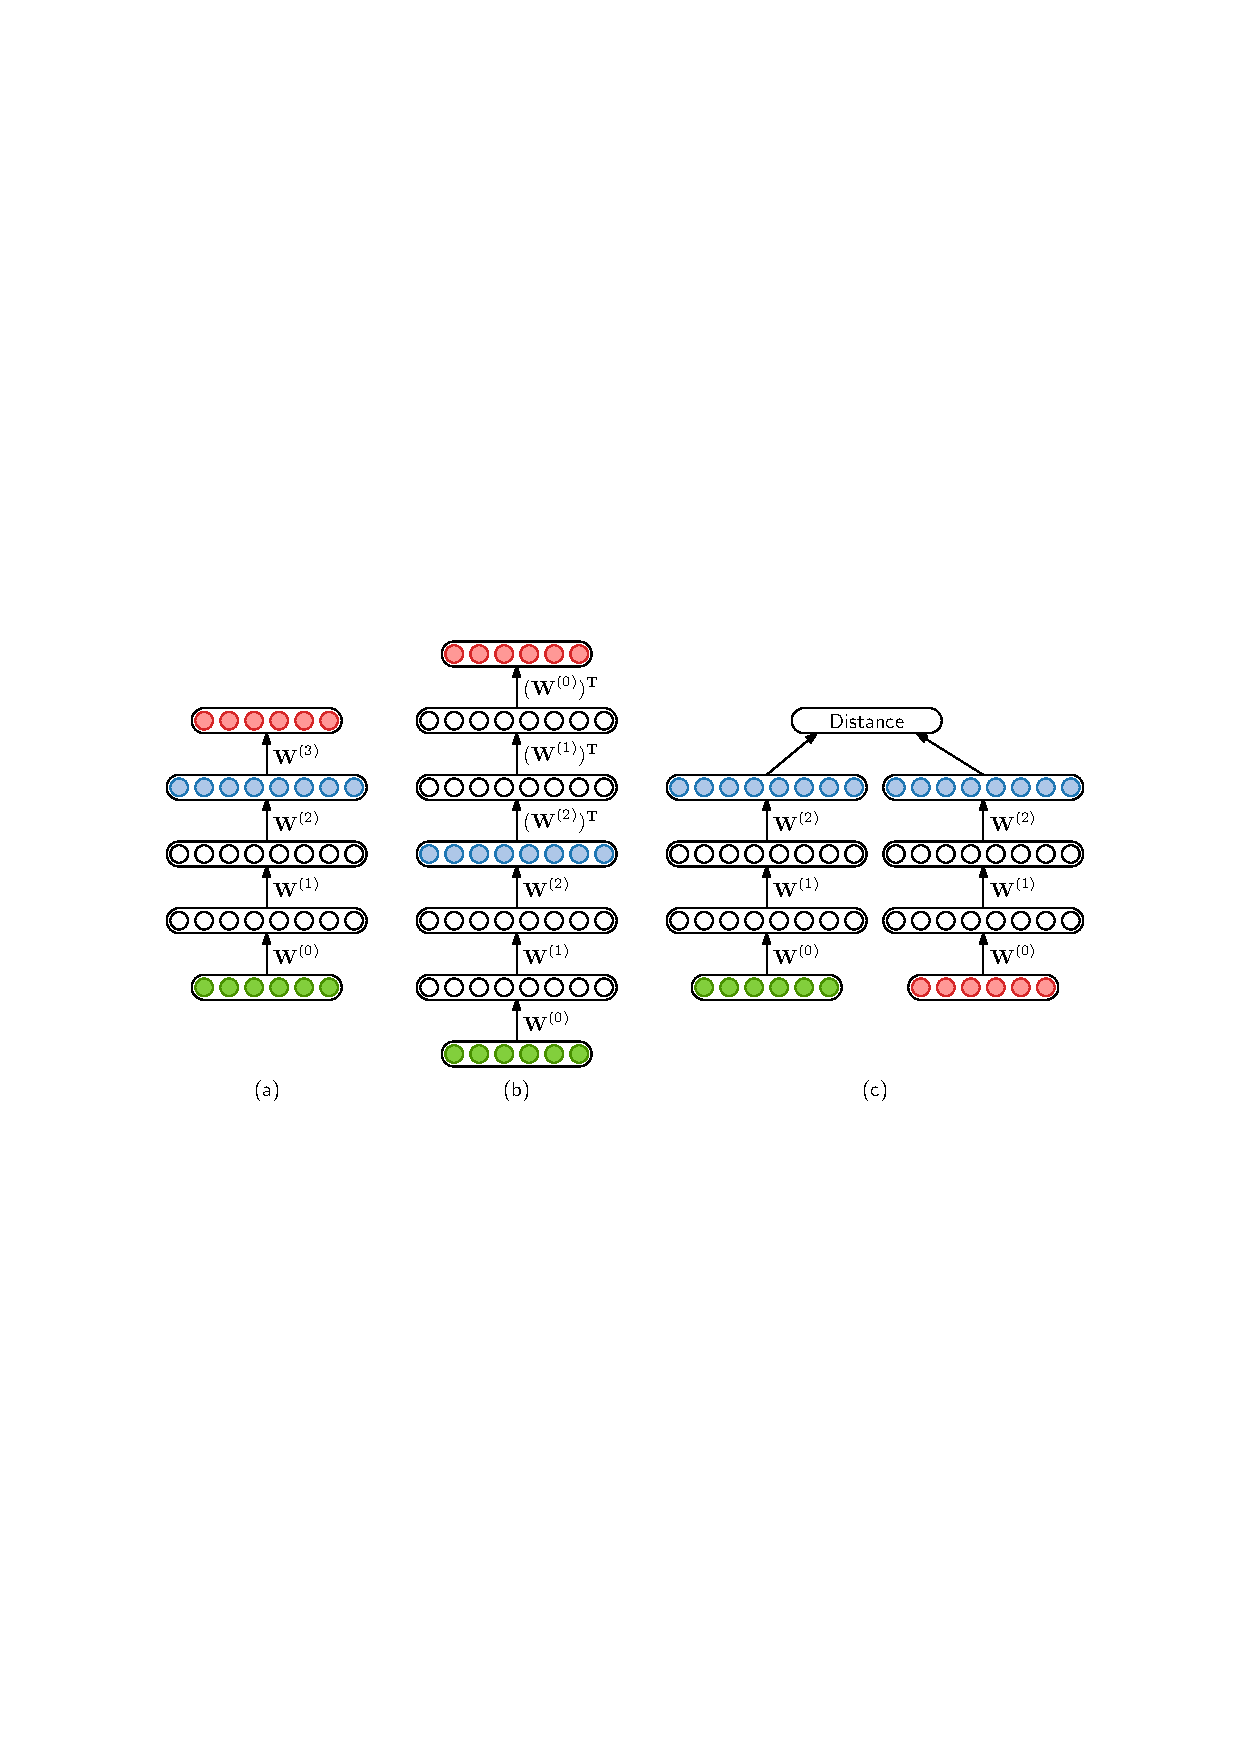
\includegraphics[width=\linewidth]{cae_siamese}
    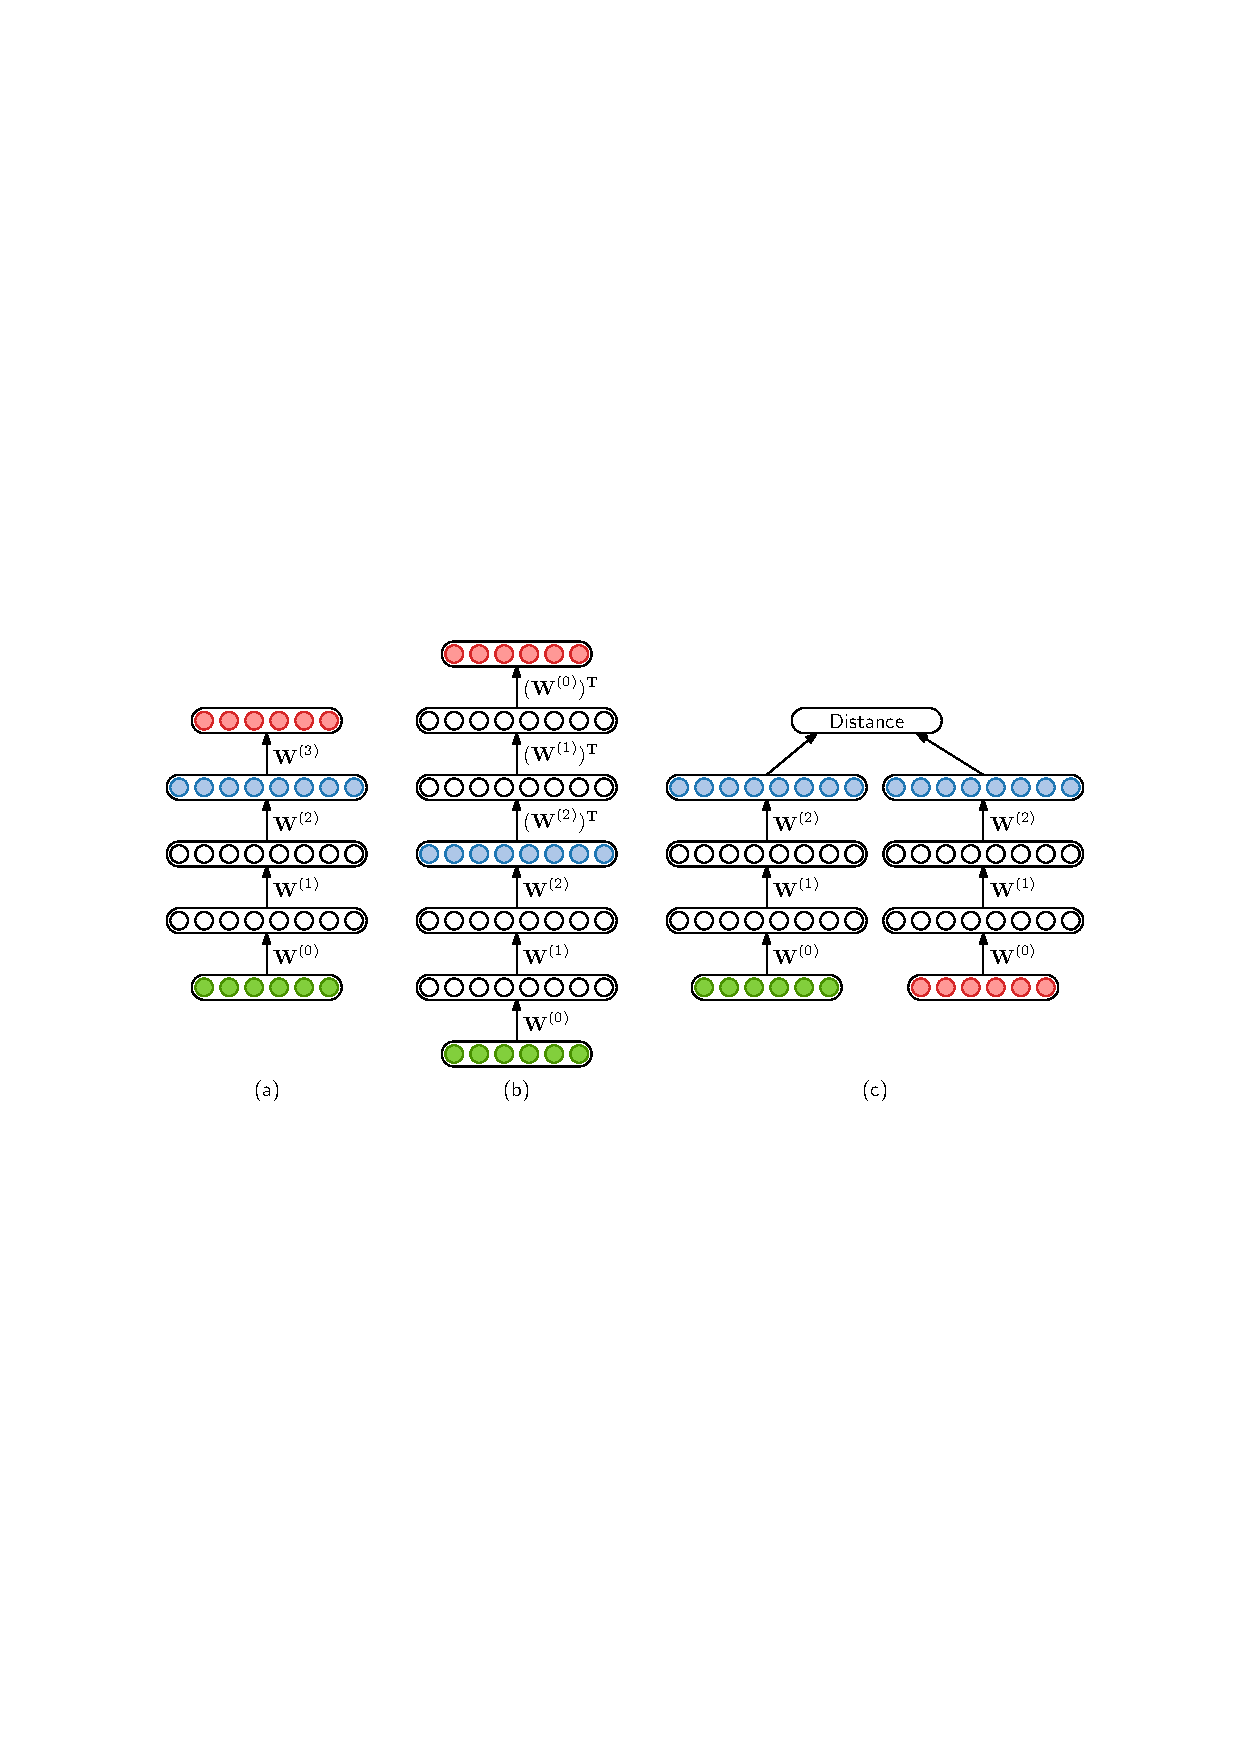
\includegraphics[width=0.918\linewidth]{cae_siamese}
    \caption[I am the short caption that appears in the list of figures, without references.]{
    (a) The cAE as used in this chapter. The encoding layer (blue) is chosen based on performance on a development set.
    (b) The cAE with symmetrical tied weights. The encoding from the middle layer (blue) is always used.
    (c) The siamese DNN. The cosine distance between aligned frames (green and red) is either minimized or maximized depending on whether the frames belong to the same (discovered) word or not.
    A cAE can be seen as a type of 
    }
    \label{fig:cae_siamese}
\end{figure}


The following is an example of an equation:
\begin{equation}
P(\vec{z} | \vec{\alpha}) = \int_{\vec{\pi}} P(\vec{z} | \vec{\pi}) \, p(\vec{\pi} | \vec{\alpha}) \, \textrm{d} \vec{\pi}
= \int_{\vec{\pi}} \prod_{k = 1}^K \pi_k^{N_k} \frac{1}{B(\vec{\alpha})} \prod_{k = 1}^K \pi_k^{\alpha_k - 1} \, \textrm{d} \vec{\pi}
\label{eq:example_equation}
\end{equation}
which you can subsequently refer to as~\eqref{eq:example_equation} or Equation~\ref{eq:example_equation}.
But make sure to consistently use the one or the other (and not mix the two ways of referring to equations).
